\documentclass[a4paper,12pt]{article}
\usepackage{float}
\usepackage[table]{xcolor} % Para colorir as linhas da tabela
\usepackage{array} % Para melhorar a formatação de tabelas
\usepackage[brazil]{babel}
\usepackage[utf8]{inputenc}
\usepackage{indentfirst}
\usepackage{amsmath}
\usepackage{multicol}
\usepackage{graphicx}
\usepackage{animate}
\usepackage{tabularx}
\usepackage[font=footnotesize, labelfont=bf, listformat=empty]{caption}
\usepackage{geometry}
\usepackage{listings}
\usepackage{lastpage}
\usepackage{subcaption}
\usepackage[skins,xparse,breakable]{tcolorbox}
\usepackage{longtable}
\usepackage{minted}
\usepackage{titlesec}
\usepackage{fancyhdr}
\usepackage{setspace}
\usepackage[colorlinks=true, allcolors=black]{hyperref}

% Configurações de margens e espaçamento
\geometry{a4paper, left=2.5cm, right=2.5cm, top=2.5cm, bottom=2cm}
\onehalfspacing

% Configurações de títulos
\titleformat{\section}{\normalfont\large\bfseries}{\thesection}{1em}{}
\titleformat{\subsection}{\normalfont\bfseries}{\thesubsection}{1em}{}
\titleformat{\subsubsection}{\normalfont\itshape}{\thesubsubsection}{1em}{}

% Configurações de listagens
\renewcommand{\listingscaption}{Código}
\newenvironment{code}{\captionsetup{type=listing}}{}

% Configurações de cores
\definecolor{LightSeaGreen}{rgb}{0.1255, 0.6980, 0.6667}
\definecolor{whitesmoke}{rgb}{0.96, 0.96, 0.96}
\definecolor{cinza}{RGB}{160, 160, 160}
\definecolor{cinza_claro}{RGB}{240, 240, 240} % Cinza claro

% Configurações do minted para VHDL
\setminted[VHDL]{
    fontsize=\footnotesize,
    style=vs,
    linenos=true,
    breaklines=true,
    mathescape=true,
    bgcolor=cinza_claro,
    breakanywhere=true,
}

\newcommand{\hex}[1]{\textcolor{green!50!black}{#1}}

% Configurações de cabeçalho e rodapé
\pagestyle{fancy}
\fancyhf{}
\fancyhead[L]{\footnotesize{Laboratório de Sistemas Digitais - ENE0040}}
\fancyhead[R]{\footnotesize{2025/1 - Turma 07}}
\fancyfoot[R]{\footnotesize{Página \hspace{0.05cm} \thepage \hspace{0.05cm} de \pageref{LastPage}}}
\fancyfoot[L]{\footnotesize{Relatório do Experimento 4}}

% Adiciona uma linha preta acima do rodapé
\renewcommand{\footrulewidth}{0.4pt} % Espessura da linha
\renewcommand{\footrule}{\vbox to 0pt{\hrule width \textwidth height \footrulewidth \vss}} % Desenha a linha

% Novo Comando para chamar a capa
\newcommand{\capa}{
    \begin{titlepage}
        \begin{multicols}{2}
            \begin{flushleft}
                
\includegraphics[width=0.45\linewidth]{Recursos/Imagens/UnB_logo.png}
            \end{flushleft}
            \columnbreak
            \begin{flushright}
                Universidade de Brasília \\
                Faculdade de Tecnologia \\
                Departamento de Engenharia Elétrica
            \end{flushright}
        \end{multicols}
        \begin{center}
        \vspace{-20pt}
        \rule{\textwidth}{0.4pt}
        \end{center}
        \vspace{0.6cm}
        \begin{center}
            {\Huge \textbf{Relatório do Experimento 4}} \\[1em]
            {\large \textbf{Autor:} Henrique Morcelles Salum} \\[0.5em]
            {\large \textbf{Matrícula:} 232003008} \\
            \vfill
            {\large \textbf{ENE0040 - Laboratório de Sistemas Digitais - Turma 07}} \\
        \end{center}
    \end{titlepage}
}

\begin{document}

\capa

% Sumário
\newpage
\tableofcontents
\newpage

% Introdução
\section{Introdução}

\subsection{Sobre o Experimento}
Este experimento é composto por duas tarefas; em ambas, deve-se implementar funções lógicas com VHDL e simulá-las por meio do software ModelSim, da Intel. É importante notar que utilizamos o \textit{top module} nesta implementação, isto é, além dos circuitos referentes às questões e dos \textit{testbenches}, criamos mais um arquivo em que instanciamos e conectamos os estímulos do \textit{testbench} e o sistema da questão. As especificidades de cada tarefa serão exploradas a seguir.

\subsubsection{Primeira Tarefa}
Na primeira tarefa, devemos implementar um dispositivo com três bits de entrada, $A$, $B$ e $C$ e dois bits de saída $X$ e $Y$. A lógica que relaciona as entradas e saídas desse dispositivo é explicitada pelas funções booleanas a seguir.
\begin{align*}
X=\overline{A}BC + A \overline{B} \hspace{0.05cm} \overline{C} + AB \\
Y= \overline{A} \hspace{0.05cm} \overline{B} + \overline{A} B \overline{C} + ABC
\end{align*}
A tabela-verdade desse dispositivo está exibida a seguir.

\begin{table}[H]
    \centering
    \footnotesize
    \begin{tabular}{|c|c|c|c|c|}
        \hline
        \rowcolor{black}
        \multicolumn{3}{|c|}{\textbf{\textcolor{white}{Entradas}}} & \multicolumn{2}{|c|}{\textbf{\textcolor{white}{Saídas}}} \\ \hline
        \rowcolor{black}
        \textcolor{white}{$A$} & \textcolor{white}{$B$} & \textcolor{white}{$C$} & \textcolor{white}{$X$} & \textcolor{white}{$Y$} \\ \hline
        0 & 0 & 0 & 0 & 1 \\ \hline
        \rowcolor{cinza}
        0 & 0 & 1 & 0 & 1 \\ \hline
        0 & 1 & 0 & 0 & 1 \\ \hline
        \rowcolor{cinza}
        0 & 1 & 1 & 1 & 0 \\ \hline
        1 & 0 & 0 & 1 & 0 \\ \hline
        \rowcolor{cinza}
        1 & 0 & 1 & 0 & 0 \\ \hline
        1 & 1 & 0 & 1 & 0 \\ \hline
        \rowcolor{cinza}
        1 & 1 & 1 & 1 & 1 \\ \hline
    \end{tabular}
    \caption{Tabela-verdade do dispositivo da questão 1}
    \label{tab: q1_1}
    \vspace{-5pt}
\end{table}


Para implementá-las, podemos utilizar apenas dois multiplexadores 4 para 1 (dispositivo desenvolvido no experimento 2) e uma porta inversora.


\subsubsection{Segunda Tarefa}

Na segunda tarefa, o dispositivo que devemos implementar em VHDL e simular no ModelSim tem sete bits de entrada, $A$, $B$, $C$, $D$, $E$, $F$ e $G$, e um bit de saída $S$. A lógica entrada-saída desse dispositivo é estabelecida de acordo com a equação a seguir.
\begin{align*}
S = &FG + 
ABCD\overline{E} \hspace{0.05cm} \overline{F}G +
\overline{A} \hspace{0.05cm} \overline{B} \hspace{0.05cm} \overline{C} \hspace{0.05cm} \overline{D} \hspace{0.05cm} \overline{E} \hspace{0.05cm} \overline{F} G +
A \overline{B} C D E F \overline{G} \hspace{0.05cm} \\
&+ \overline{A} B C D \overline{E} F \overline{G} +
A B C D E \overline{F}  \hspace{0.05cm}  \overline{G} +
A \overline{B} \hspace{0.05cm} \overline{C} D E \overline{F} \hspace{0.05cm} \overline{G}
\end{align*}


Para melhor apresentação desse documento, não exibiremos a tabela-verdade desse dispositivo, que teria 128 linhas. Ao invés disso, representaremos a função como o somatório dos mintermos que a formam.
\begin{equation} \label{eq: q2}
\sum_{A,C,D,E,F,G} \substack{m(1,3,7,11,15,19,23,27,31,35,39,43,47,51,55,58,59,63,
67,71,\\75,76,79,83,87,91,95,99,103,107,111,115,119,121,123,124,127)}
\end{equation}


Para implementar esse dispositivo, nos é permitida a utilização de um decodificador 4 para 16, um multiplexador 8 para 1 (sistemas desenvolvidos no experimento 3) e três portas `OU'.

\subsection{Introdução Teórica}
 Ambos os dispositivos utilizados nesse experimento - multiplexador e decodificador - já foram extensivamente explicados nos relatórios anteriores. Aqui, portanto, a explicação será breve: só nos interessa lembrar que, no multiplexador, as entradas de dados podem servir para implementar funções das entradas de seleção e que cada saída do decodificador é um dos $2^n$ mintermos das suas $n$ entradas. Como essas propriedades serão utilizadas na realização de cada tarefa aqui discutida, está explicado nas próximas seções.

\subsubsection{Primeira Tarefa}

Nessa tarefa, só nos é permitida a utilização de dois multiplexadores 4 para 1 - dotados de duas entradas de seleção cada - implementados em VHDL pelo código a seguir.
\begin{code}
\begin{minted}{VHDL}
library IEEE;
use IEEE.std_logic_1164.all;

entity Mux4x1 is
    port (
        D: in std_logic_vector(3 downto 0);
        S: in std_logic_vector(1 downto 0);
        Y: out std_logic -- Saída
    );
end entity Mux4x1;

architecture behavioral of Mux4x1 is
begin
    Y <= D(3) when (S = "11") else
         D(2) when (S = "10") else
         D(1) when (S = "01") else
         D(0) when (S = "00") else
         '-';
end architecture behavioral;
\end{minted}
\caption{Código para implementação do multiplexador 4 para 1}
\end{code}


Note, porém, que as funções $X$ e $Y$ que precisamos implementar nesse dispositivo dependem de três variáveis. Nesse caso, podemos introduzir uma das entradas nas saídas, como mostra a tabela-verdade a seguir.

\begin{table}[H] \label{tab: q1}
    \centering
    \renewcommand{\arraystretch}{1.5} % Aumenta o espaçamento vertical das linhas
    \begin{tabular}{|>{\centering\arraybackslash}p{0.75cm}|>{\centering\arraybackslash}p{0.75cm}|>{\centering\arraybackslash}p{1cm}|>{\centering\arraybackslash}p{1cm}|}
        \hline
        \rowcolor{black}
        \multicolumn{2}{|c|}{\textbf{\textcolor{white}{Entradas}}} & \multicolumn{2}{|c|}{\textbf{\textcolor{white}{Saídas}}} \\ \hline
        \rowcolor{black}
        \textcolor{white}{$A$} & \textcolor{white}{$B$} & \textcolor{white}{$X(C)$} & \textcolor{white}{$Y(C)$} \\ \hline
        0 & 0 & 0 & 1 \\ \hline
        \rowcolor{cinza}
        0 & 1 & $C$ & $\overline{C}$ \\ \hline
        1 & 0 & $\overline{C}$ & 0 \\ \hline
        \rowcolor{cinza}
        1 & 1 & 1 & $C$ \\ \hline
    \end{tabular}
    \caption{Tabela-verdade do dispositivo da questão 1}
    \vspace{-5pt}
\end{table}


No circuito, isso significa inserir a entrada $C$ nas entradas de dados do multiplexador, como mostra a figura a seguir.

\begin{figure}[H]
    \centering
    \scalebox{0.6}{
\begin{tikzpicture}[x=1pt,y=-1pt,line cap=rect]
\useasboundingbox (0,0) rectangle (235,450);
\def\logisimfontA#1{\fontfamily{cmr}{#1}} % Replaced by logisim, original font was "SansSerif"
\def\logisimfontB#1{\fontfamily{Dialog}{#1}}
\def\logisimfontC#1{\fontfamily{Ubuntu}{#1}}
\definecolor{custcol_0_0_0}{RGB}{0, 0, 0}
\definecolor{custcol_ff_ff_ff}{RGB}{255, 255, 255}
\draw [line width=3.0pt, custcol_0_0_0 ]  (165.0,148.0) -- (215.0,148.0) ;
\draw [line width=3.0pt, custcol_0_0_0 ]  (165.0,368.0) -- (215.0,368.0) ;
\draw [line width=4.0pt, custcol_0_0_0 ]  (125.0,218.0) -- (125.0,238.0) ;
\draw [line width=4.0pt, custcol_0_0_0 ]  (125.0,438.0) -- (125.0,458.0) ;
\draw [line width=3.0pt, custcol_0_0_0 ]  (45.0,168.0) -- (85.0,168.0) ;
\draw [line width=3.0pt, custcol_0_0_0 ]  (45.0,348.0) -- (85.0,348.0) ;
\draw [line width=3.0pt, custcol_0_0_0 ]  (85.0,88.0) -- (55.0,88.0) -- (55.0,388.0) ;
\draw [line width=3.0pt, custcol_0_0_0 ]  (65.0,208.0) -- (85.0,208.0) ;
\draw [line width=3.0pt, custcol_0_0_0 ]  (15.0,168.0) -- (25.0,168.0) ;
\draw [line width=3.0pt, custcol_0_0_0 ]  (15.0,348.0) -- (25.0,348.0) ;
\draw [line width=3.0pt, custcol_0_0_0 ]  (15.0,128.0) -- (85.0,128.0) ;
\draw [line width=3.0pt, custcol_0_0_0 ]  (15.0,48.0) -- (15.0,128.0) -- (15.0,168.0) -- (15.0,348.0) -- (15.0,428.0) -- (85.0,428.0) ;
\fill [line width=3.0pt, custcol_0_0_0]  (15.0,128.0) ellipse (5.0 and 5.0 );
\fill [line width=3.0pt, custcol_0_0_0]  (55.0,388.0) ellipse (5.0 and 5.0 );
\fill [line width=3.0pt, custcol_0_0_0]  (15.0,348.0) ellipse (5.0 and 5.0 );
\fill [line width=3.0pt, custcol_0_0_0]  (65.0,208.0) ellipse (5.0 and 5.0 );
\fill [line width=3.0pt, custcol_0_0_0]  (15.0,168.0) ellipse (5.0 and 5.0 );
\draw [line width=2.0pt, custcol_0_0_0 ]  (39.0,168.0) -- (26.0,162.0) -- (26.0,174.0) -- cycle;
\draw [line width=2.0pt, custcol_0_0_0]  (42.0,168.0) ellipse (3.0 and 3.0 );
\fill [line width=2.0pt, custcol_0_0_0]  (45.0,168.0) ellipse (2.0 and 2.0 );
\fill [line width=2.0pt, custcol_0_0_0]  (25.0,168.0) ellipse (2.0 and 2.0 );
\draw [line width=3.0pt, custcol_0_0_0 ]  (85.0,308.0) -- (65.0,308.0) -- (65.0,208.0) -- (65.0,48.0) -- (65.0,43.0) ;
\draw [line width=1.0pt, custcol_0_0_0 ]  (57.0,42.0) -- (65.0,34.0) -- (73.0,42.0) -- cycle;
\fill [line width=1.0pt, custcol_0_0_0]  (65.0,48.0) ellipse (2.0 and 2.0 );
\logisimfontB{\fontsize{14pt}{14pt}\fontseries{bx}\selectfont\node[inner sep=0, outer sep=0, custcol_0_0_0, anchor=base west] at  (147.0,155.0)  {Y};}
\draw [line width=5.0pt, custcol_0_0_0 ]  (85.0,58.0) -- (85.0,239.0) -- (165.0,198.0) -- (165.0,99.0) -- cycle;
\logisimfontB{\fontsize{16pt}{16pt}\fontseries{bx}\selectfont\node[inner sep=0, outer sep=0, custcol_0_0_0, anchor=base west] at  (94.0,95.0)  {0};}
\logisimfontC{\fontsize{16pt}{16pt}\fontseries{bx}\selectfont\node[inner sep=0, outer sep=0, custcol_0_0_0, anchor=base west] at  (120.0,210.0)  {S};}
\fill [line width=1.0pt, custcol_0_0_0]  (85.0,88.0) ellipse (2.0 and 2.0 );
\fill [line width=1.0pt, custcol_0_0_0]  (85.0,128.0) ellipse (2.0 and 2.0 );
\fill [line width=1.0pt, custcol_0_0_0]  (85.0,168.0) ellipse (2.0 and 2.0 );
\fill [line width=1.0pt, custcol_0_0_0]  (85.0,208.0) ellipse (2.0 and 2.0 );
\fill [line width=1.0pt, custcol_0_0_0]  (125.0,218.0) ellipse (2.0 and 2.0 );
\fill [line width=1.0pt, custcol_0_0_0]  (165.0,148.0) ellipse (2.0 and 2.0 );
\draw [line width=2.0pt, custcol_0_0_0 ]  (7.0,30.0) -- (24.0,30.0) ;
\draw [line width=2.0pt, custcol_0_0_0 ]  (25.0,30.0) -- (25.0,47.0) ;
\draw [line width=2.0pt, custcol_0_0_0 ]  (25.0,48.0) -- (8.0,48.0) ;
\draw [line width=2.0pt, custcol_0_0_0 ]  (7.0,48.0) -- (7.0,31.0) ;
\logisimfontA{\fontsize{12pt}{12pt}\selectfont\node[inner sep=0, outer sep=0, custcol_0_0_0, anchor=base west] at  (9.0,45.0)  {x1};}
\logisimfontA{\fontsize{16pt}{16pt}\fontseries{bx}\selectfont\node[inner sep=0, outer sep=0, custcol_0_0_0, anchor=base west] at  (10.0,22.0)  {C};}
\fill [line width=2.0pt, custcol_0_0_0]  (15.0,48.0) ellipse (2.0 and 2.0 );
\logisimfontA{\fontsize{16pt}{16pt}\fontseries{bx}\selectfont\node[inner sep=0, outer sep=0, custcol_0_0_0, anchor=base west] at  (120.0,259.0)  {S};}
\draw [line width=2.0pt, custcol_0_0_0 ]  (117.0,242.0) -- (125.0,238.0) -- (133.0,242.0) -- (133.0,267.0) -- (117.0,267.0) -- cycle;
\fill [line width=2.0pt, custcol_0_0_0]  (125.0,238.0) ellipse (2.0 and 2.0 );
\draw [line width=2.0pt, custcol_0_0_0 ]  (217.0,30.0) -- (234.0,30.0) ;
\draw [line width=2.0pt, custcol_0_0_0 ]  (235.0,30.0) -- (235.0,47.0) ;
\draw [line width=2.0pt, custcol_0_0_0 ]  (235.0,48.0) -- (218.0,48.0) ;
\draw [line width=2.0pt, custcol_0_0_0 ]  (217.0,48.0) -- (217.0,31.0) ;
\logisimfontA{\fontsize{12pt}{12pt}\selectfont\node[inner sep=0, outer sep=0, custcol_0_0_0, anchor=base west] at  (219.0,45.0)  {x1};}
\logisimfontA{\fontsize{16pt}{16pt}\fontseries{bx}\selectfont\node[inner sep=0, outer sep=0, custcol_0_0_0, anchor=base west] at  (220.0,22.0)  {B};}
\fill [line width=2.0pt, custcol_0_0_0]  (225.0,48.0) ellipse (2.0 and 2.0 );
\draw [line width=2.0pt, custcol_0_0_0 ]  (187.0,30.0) -- (204.0,30.0) ;
\draw [line width=2.0pt, custcol_0_0_0 ]  (205.0,30.0) -- (205.0,47.0) ;
\draw [line width=2.0pt, custcol_0_0_0 ]  (205.0,48.0) -- (188.0,48.0) ;
\draw [line width=2.0pt, custcol_0_0_0 ]  (187.0,48.0) -- (187.0,31.0) ;
\logisimfontA{\fontsize{12pt}{12pt}\selectfont\node[inner sep=0, outer sep=0, custcol_0_0_0, anchor=base west] at  (189.0,45.0)  {x1};}
\logisimfontA{\fontsize{16pt}{16pt}\fontseries{bx}\selectfont\node[inner sep=0, outer sep=0, custcol_0_0_0, anchor=base west] at  (190.0,22.0)  {A};}
\fill [line width=2.0pt, custcol_0_0_0]  (195.0,48.0) ellipse (2.0 and 2.0 );
\logisimfontA{\fontsize{16pt}{16pt}\fontseries{bx}\selectfont\node[inner sep=0, outer sep=0, custcol_0_0_0, anchor=base west] at  (210.0,99.0)  {S};}
\draw [line width=2.0pt, custcol_0_0_0 ]  (207.0,82.0) -- (215.0,78.0) -- (223.0,82.0) -- (223.0,107.0) -- (207.0,107.0) -- cycle;
\fill [line width=2.0pt, custcol_0_0_0]  (215.0,78.0) ellipse (2.0 and 2.0 );
\draw [line width=3.0pt, custcol_0_0_0 ]  (225.0,48.0) -- (225.0,58.0) -- (215.0,58.0) -- (215.0,72.0) ;
\draw [line width=3.0pt, custcol_0_0_0 ]  (195.0,48.0) -- (195.0,58.0) -- (205.0,58.0) -- (205.0,72.0) ;
\draw [line width=5.0pt, custcol_0_0_0 ]  (215.0,77.0) -- (215.0,72.0) ;
\draw [line width=5.0pt, custcol_0_0_0 ]  (214.0,72.0) -- (206.0,72.0) ;
\logisimfontA{\fontsize{7pt}{7pt}\selectfont\node[inner sep=0, outer sep=0, custcol_0_0_0, anchor=base west, rotate=-90.0] at  (218.0,65.0)  {0};}
\logisimfontA{\fontsize{7pt}{7pt}\selectfont\node[inner sep=0, outer sep=0, custcol_0_0_0, anchor=base west, rotate=-90.0] at  (208.0,65.0)  {1};}
\fill [line width=5.0pt, custcol_0_0_0]  (215.0,78.0) ellipse (2.0 and 2.0 );
\fill [line width=5.0pt, custcol_0_0_0]  (215.0,58.0) ellipse (2.0 and 2.0 );
\fill [line width=5.0pt, custcol_0_0_0]  (205.0,58.0) ellipse (2.0 and 2.0 );
\draw [line width=2.0pt, custcol_0_0_0]  (226.0,149.0) ellipse (9.0 and 9.0 );
\logisimfontA{\fontsize{12pt}{12pt}\selectfont\node[inner sep=0, outer sep=0, custcol_0_0_0, anchor=base west] at  (219.0,155.0)  {x1};}
\logisimfontA{\fontsize{16pt}{16pt}\fontseries{bx}\selectfont\node[inner sep=0, outer sep=0, custcol_0_0_0, anchor=base west] at  (237.0,156.0)  {X};}
\fill [line width=2.0pt, custcol_0_0_0]  (215.0,148.0) ellipse (2.0 and 2.0 );
\draw [line width=2.0pt, custcol_0_0_0 ]  (39.0,348.0) -- (26.0,342.0) -- (26.0,354.0) -- cycle;
\draw [line width=2.0pt, custcol_0_0_0]  (42.0,348.0) ellipse (3.0 and 3.0 );
\fill [line width=2.0pt, custcol_0_0_0]  (45.0,348.0) ellipse (2.0 and 2.0 );
\fill [line width=2.0pt, custcol_0_0_0]  (25.0,348.0) ellipse (2.0 and 2.0 );
\logisimfontB{\fontsize{14pt}{14pt}\fontseries{bx}\selectfont\node[inner sep=0, outer sep=0, custcol_0_0_0, anchor=base west] at  (147.0,375.0)  {Y};}
\draw [line width=5.0pt, custcol_0_0_0 ]  (85.0,278.0) -- (85.0,459.0) -- (165.0,418.0) -- (165.0,319.0) -- cycle;
\logisimfontB{\fontsize{16pt}{16pt}\fontseries{bx}\selectfont\node[inner sep=0, outer sep=0, custcol_0_0_0, anchor=base west] at  (94.0,315.0)  {0};}
\logisimfontC{\fontsize{16pt}{16pt}\fontseries{bx}\selectfont\node[inner sep=0, outer sep=0, custcol_0_0_0, anchor=base west] at  (120.0,430.0)  {S};}
\fill [line width=1.0pt, custcol_0_0_0]  (85.0,308.0) ellipse (2.0 and 2.0 );
\fill [line width=1.0pt, custcol_0_0_0]  (85.0,348.0) ellipse (2.0 and 2.0 );
\fill [line width=1.0pt, custcol_0_0_0]  (85.0,388.0) ellipse (2.0 and 2.0 );
\fill [line width=1.0pt, custcol_0_0_0]  (85.0,428.0) ellipse (2.0 and 2.0 );
\fill [line width=1.0pt, custcol_0_0_0]  (125.0,438.0) ellipse (2.0 and 2.0 );
\fill [line width=1.0pt, custcol_0_0_0]  (165.0,368.0) ellipse (2.0 and 2.0 );
\logisimfontA{\fontsize{16pt}{16pt}\fontseries{bx}\selectfont\node[inner sep=0, outer sep=0, custcol_0_0_0, anchor=base west] at  (120.0,479.0)  {S};}
\draw [line width=2.0pt, custcol_0_0_0 ]  (117.0,462.0) -- (125.0,458.0) -- (133.0,462.0) -- (133.0,487.0) -- (117.0,487.0) -- cycle;
\fill [line width=2.0pt, custcol_0_0_0]  (125.0,458.0) ellipse (2.0 and 2.0 );
\draw [line width=2.0pt, custcol_0_0_0]  (226.0,369.0) ellipse (9.0 and 9.0 );
\logisimfontA{\fontsize{12pt}{12pt}\selectfont\node[inner sep=0, outer sep=0, custcol_0_0_0, anchor=base west] at  (219.0,375.0)  {x1};}
\logisimfontA{\fontsize{16pt}{16pt}\fontseries{bx}\selectfont\node[inner sep=0, outer sep=0, custcol_0_0_0, anchor=base west] at  (237.0,376.0)  {Y};}
\fill [line width=2.0pt, custcol_0_0_0]  (215.0,368.0) ellipse (2.0 and 2.0 );
\draw [line width=3.0pt, custcol_0_0_0 ]  (85.0,388.0) -- (55.0,388.0) -- (55.0,468.0) -- (55.0,473.0) ;
\draw [line width=1.0pt, custcol_0_0_0 ]  (63.0,474.0) -- (47.0,474.0) ;
\draw [line width=1.0pt, custcol_0_0_0 ]  (60.0,477.0) -- (50.0,477.0) ;
\draw [line width=1.0pt, custcol_0_0_0 ]  (57.0,480.0) -- (53.0,480.0) ;
\fill [line width=1.0pt, custcol_0_0_0]  (55.0,468.0) ellipse (2.0 and 2.0 );
\end{tikzpicture}
}
    \caption{Implementação do dispositivo da questão 1 com a variável $C$ inserida}
    \label{fig:enter-label}
\end{figure}


Sem nenhuma razão além de facilidade de compreensão, escolhemos introduzir o $C$, mas poderíamos, sem nenhum prejuízo, introduzir o $A$ ou o $B$. Nesses casos, seria conveniente reorientar a tabela-verdade original para facilitar a inserção da variável escolhida na saída, mas é claro que isso não geraria nenhum prejuízo ao sistema.

\subsubsection{Segunda Tarefa}

Nessa questão, somos restritos a utilizar um multiplexador 8 para 1 e um decodificador 4 para 16, implementados como segue.
\begin{figure}[htbp]
    \centering
    \begin{minipage}[t]{0.49\textwidth}
        \centering
        \begin{code}
            \begin{minted}[fontsize=\footnotesize, linenos=false]{VHDL}
library IEEE;
use IEEE.std_logic_1164.all;

entity Mux8x1 is
    port (
        D: in std_logic_vector(7 downto 0);
        S: in std_logic_vector(2 downto 0);
        Y: out std_logic
    );
end entity Mux8x1;

architecture behavioral of Mux8x1 is
begin
    Y <= D(7) when (S = "111") else
         D(6) when (S = "110") else
         D(5) when (S = "101") else
         D(4) when (S = "100") else
         D(3) when (S = "011") else
         D(2) when (S = "010") else
         D(1) when (S = "001") else
         D(0) when (S = "000") else
         '-';    
end architecture behavioral;
            \end{minted}
            \caption{Mux 8x1}
            \label{fig:mux8x1}
        \end{code}
    \end{minipage}
    \hfill
    \begin{minipage}[t]{0.49\textwidth}
        \centering
        \begin{code}
            \begin{minted}[escapeinside=||,fontsize=\scriptsize, linenos=false]{VHDL}
library IEEE;
use IEEE.std_logic_1164.all;

entity Dec4x16 is
    port (
        A: in std_logic_vector(3 downto 0);
        Y: out std_logic_vector(15 downto 0)
    );
end entity Dec4x16;

architecture behavioral of Dec4x16 is
begin
    with A select Y <=
        |\hex{X"0001"}| when |\hex{X"0"}|,
        |\hex{X"0002"}| when |\hex{X"1"}|,
        |\hex{X"0004"}| when |\hex{X"2"}|,
        |\hex{X"0008"}| when |\hex{X"3"}|,
        |\hex{X"0010"}| when |\hex{X"4"}|,
        |\hex{X"0020"}| when |\hex{X"5"}|,
        |\hex{X"0040"}| when |\hex{X"6"}|,
        |\hex{X"0080"}| when |\hex{X"7"}|,
        |\hex{X"0100"}| when |\hex{X"8"}|,
        |\hex{X"0200"}| when |\hex{X"9"}|,
        |\hex{X"0400"}| when |\hex{X"A"}|,
        |\hex{X"0800"}| when |\hex{X"B"}|,
        |\hex{X"1000"}| when |\hex{X"C"}|,
        |\hex{X"2000"}| when |\hex{X"D"}|,
        |\hex{X"4000"}| when |\hex{X"E"}|,
        |\hex{X"8000"}| when |\hex{X"F"}|,
        "----------------" when others;
end architecture behavioral;
            \end{minted}
            \caption{Dec 4x16}
            \label{fig:dec4x16}
        \end{code}
    \end{minipage}
\end{figure}


O problema é o parecido com o da questão anterior: um decodificador 4 para 16 gera todos os mintermos de \textbf{quatro} variáveis, mas temos sete! Aqui podemos utilizar o multiplexador para resolver esse problema: fazemos das outras três variáveis as entradas de seleção do multiplexador 8 para 1 e conseguimos implementar a função.

\begin{figure}[H]
    \centering
    \scalebox{0.7}{
\begin{tikzpicture}[x=1pt,y=-1pt,line cap=rect]
\useasboundingbox (0,0) rectangle (410,210);
\def\logisimfontA#1{\fontfamily{cmr}{#1}} % Replaced by logisim, original font was "SansSerif"
\def\logisimfontB#1{\fontfamily{Lexend}{#1}}
\definecolor{custcol_0_0_0}{RGB}{0, 0, 0}
\definecolor{custcol_ff_ff_ff}{RGB}{255, 255, 255}
\draw [line width=3.0pt, custcol_0_0_0 ]  (228.0,120.0) -- (278.0,120.0) ;
\draw [line width=3.0pt, custcol_0_0_0 ]  (358.0,110.0) -- (398.0,110.0) ;
\draw [line width=3.0pt, custcol_0_0_0 ]  (298.0,190.0) -- (298.0,210.0) ;
\draw [line width=3.0pt, custcol_0_0_0 ]  (318.0,180.0) -- (318.0,210.0) ;
\draw [line width=3.0pt, custcol_0_0_0 ]  (338.0,170.0) -- (338.0,210.0) ;
\draw [line width=3.0pt, custcol_0_0_0 ]  (38.0,40.0) -- (68.0,40.0) ;
\draw [line width=3.0pt, custcol_0_0_0 ]  (38.0,90.0) -- (68.0,90.0) ;
\draw [line width=3.0pt, custcol_0_0_0 ]  (38.0,140.0) -- (68.0,140.0) ;
\draw [line width=3.0pt, custcol_0_0_0 ]  (38.0,190.0) -- (68.0,190.0) ;
\draw [line width=3.0pt, custcol_0_0_0 ]  (248.0,100.0) -- (278.0,100.0) ;
\draw [line width=3.0pt, custcol_0_0_0 ]  (258.0,140.0) -- (278.0,140.0) ;
\draw [line width=3.0pt, custcol_0_0_0 ]  (228.0,50.0) -- (238.0,50.0) -- (238.0,60.0) -- (278.0,60.0) ;
\draw [line width=3.0pt, custcol_0_0_0 ]  (168.0,110.0) -- (178.0,110.0) -- (178.0,80.0) -- (278.0,80.0) ;
\draw [line width=3.0pt, custcol_0_0_0 ]  (168.0,150.0) -- (198.0,150.0) -- (198.0,160.0) -- (278.0,160.0) ;
\fill [line width=3.0pt, custcol_0_0_0]  (248.0,100.0) ellipse (5.0 and 5.0 );
\fill [line width=3.0pt, custcol_0_0_0]  (188.0,110.0) ellipse (5.0 and 5.0 );
\fill [line width=3.0pt, custcol_0_0_0]  (258.0,140.0) ellipse (5.0 and 5.0 );
\draw [line width=2.0pt, custcol_0_0_0 ]  (20.0,32.0) -- (37.0,32.0) ;
\draw [line width=2.0pt, custcol_0_0_0 ]  (38.0,32.0) -- (38.0,49.0) ;
\draw [line width=2.0pt, custcol_0_0_0 ]  (38.0,50.0) -- (21.0,50.0) ;
\draw [line width=2.0pt, custcol_0_0_0 ]  (20.0,50.0) -- (20.0,33.0) ;
\logisimfontA{\fontsize{12pt}{12pt}\selectfont\node[inner sep=0, outer sep=0, custcol_0_0_0, anchor=base west] at  (22.0,47.0)  {x1};}
\logisimfontA{\fontsize{16pt}{16pt}\fontseries{bx}\selectfont\node[inner sep=0, outer sep=0, custcol_0_0_0, anchor=base west] at  (6.0,48.0)  {A};}
\fill [line width=2.0pt, custcol_0_0_0]  (38.0,40.0) ellipse (2.0 and 2.0 );
\draw [line width=2.0pt, custcol_0_0_0 ]  (20.0,82.0) -- (37.0,82.0) ;
\draw [line width=2.0pt, custcol_0_0_0 ]  (38.0,82.0) -- (38.0,99.0) ;
\draw [line width=2.0pt, custcol_0_0_0 ]  (38.0,100.0) -- (21.0,100.0) ;
\draw [line width=2.0pt, custcol_0_0_0 ]  (20.0,100.0) -- (20.0,83.0) ;
\logisimfontA{\fontsize{12pt}{12pt}\selectfont\node[inner sep=0, outer sep=0, custcol_0_0_0, anchor=base west] at  (22.0,97.0)  {x1};}
\logisimfontA{\fontsize{16pt}{16pt}\fontseries{bx}\selectfont\node[inner sep=0, outer sep=0, custcol_0_0_0, anchor=base west] at  (5.0,98.0)  {B};}
\fill [line width=2.0pt, custcol_0_0_0]  (38.0,90.0) ellipse (2.0 and 2.0 );
\draw [line width=2.0pt, custcol_0_0_0 ]  (20.0,132.0) -- (37.0,132.0) ;
\draw [line width=2.0pt, custcol_0_0_0 ]  (38.0,132.0) -- (38.0,149.0) ;
\draw [line width=2.0pt, custcol_0_0_0 ]  (38.0,150.0) -- (21.0,150.0) ;
\draw [line width=2.0pt, custcol_0_0_0 ]  (20.0,150.0) -- (20.0,133.0) ;
\logisimfontA{\fontsize{12pt}{12pt}\selectfont\node[inner sep=0, outer sep=0, custcol_0_0_0, anchor=base west] at  (22.0,147.0)  {x1};}
\logisimfontA{\fontsize{16pt}{16pt}\fontseries{bx}\selectfont\node[inner sep=0, outer sep=0, custcol_0_0_0, anchor=base west] at  (5.0,148.0)  {C};}
\fill [line width=2.0pt, custcol_0_0_0]  (38.0,140.0) ellipse (2.0 and 2.0 );
\draw [line width=2.0pt, custcol_0_0_0 ]  (20.0,182.0) -- (37.0,182.0) ;
\draw [line width=2.0pt, custcol_0_0_0 ]  (38.0,182.0) -- (38.0,199.0) ;
\draw [line width=2.0pt, custcol_0_0_0 ]  (38.0,200.0) -- (21.0,200.0) ;
\draw [line width=2.0pt, custcol_0_0_0 ]  (20.0,200.0) -- (20.0,183.0) ;
\logisimfontA{\fontsize{12pt}{12pt}\selectfont\node[inner sep=0, outer sep=0, custcol_0_0_0, anchor=base west] at  (22.0,197.0)  {x1};}
\logisimfontA{\fontsize{16pt}{16pt}\fontseries{bx}\selectfont\node[inner sep=0, outer sep=0, custcol_0_0_0, anchor=base west] at  (5.0,198.0)  {D};}
\fill [line width=2.0pt, custcol_0_0_0]  (38.0,190.0) ellipse (2.0 and 2.0 );
\draw [line width=3.0pt, custcol_0_0_0 ]  (278.0,180.0) -- (248.0,180.0) -- (248.0,100.0) -- (248.0,20.0) -- (248.0,15.0) ;
\draw [line width=1.0pt, custcol_0_0_0 ]  (240.0,14.0) -- (248.0,6.0) -- (256.0,14.0) -- cycle;
\fill [line width=1.0pt, custcol_0_0_0]  (248.0,20.0) ellipse (2.0 and 2.0 );
\draw [line width=3.0pt, custcol_0_0_0 ]  (278.0,40.0) -- (258.0,40.0) -- (258.0,140.0) -- (258.0,230.0) -- (258.0,235.0) ;
\draw [line width=1.0pt, custcol_0_0_0 ]  (266.0,236.0) -- (250.0,236.0) ;
\draw [line width=1.0pt, custcol_0_0_0 ]  (263.0,239.0) -- (253.0,239.0) ;
\draw [line width=1.0pt, custcol_0_0_0 ]  (260.0,242.0) -- (256.0,242.0) ;
\fill [line width=1.0pt, custcol_0_0_0]  (258.0,230.0) ellipse (2.0 and 2.0 );
\draw [line width=2.0pt, custcol_0_0_0 ]  (290.0,212.0) -- (307.0,212.0) ;
\draw [line width=2.0pt, custcol_0_0_0 ]  (308.0,212.0) -- (308.0,229.0) ;
\draw [line width=2.0pt, custcol_0_0_0 ]  (308.0,230.0) -- (291.0,230.0) ;
\draw [line width=2.0pt, custcol_0_0_0 ]  (290.0,230.0) -- (290.0,213.0) ;
\logisimfontA{\fontsize{12pt}{12pt}\selectfont\node[inner sep=0, outer sep=0, custcol_0_0_0, anchor=base west] at  (292.0,227.0)  {x1};}
\logisimfontA{\fontsize{16pt}{16pt}\fontseries{bx}\selectfont\node[inner sep=0, outer sep=0, custcol_0_0_0, anchor=base west] at  (293.0,249.0)  {E};}
\fill [line width=2.0pt, custcol_0_0_0]  (298.0,210.0) ellipse (2.0 and 2.0 );
\draw [line width=2.0pt, custcol_0_0_0 ]  (310.0,212.0) -- (327.0,212.0) ;
\draw [line width=2.0pt, custcol_0_0_0 ]  (328.0,212.0) -- (328.0,229.0) ;
\draw [line width=2.0pt, custcol_0_0_0 ]  (328.0,230.0) -- (311.0,230.0) ;
\draw [line width=2.0pt, custcol_0_0_0 ]  (310.0,230.0) -- (310.0,213.0) ;
\logisimfontA{\fontsize{12pt}{12pt}\selectfont\node[inner sep=0, outer sep=0, custcol_0_0_0, anchor=base west] at  (312.0,227.0)  {x1};}
\logisimfontA{\fontsize{16pt}{16pt}\fontseries{bx}\selectfont\node[inner sep=0, outer sep=0, custcol_0_0_0, anchor=base west] at  (313.0,249.0)  {F};}
\fill [line width=2.0pt, custcol_0_0_0]  (318.0,210.0) ellipse (2.0 and 2.0 );
\draw [line width=2.0pt, custcol_0_0_0 ]  (330.0,212.0) -- (347.0,212.0) ;
\draw [line width=2.0pt, custcol_0_0_0 ]  (348.0,212.0) -- (348.0,229.0) ;
\draw [line width=2.0pt, custcol_0_0_0 ]  (348.0,230.0) -- (331.0,230.0) ;
\draw [line width=2.0pt, custcol_0_0_0 ]  (330.0,230.0) -- (330.0,213.0) ;
\logisimfontA{\fontsize{12pt}{12pt}\selectfont\node[inner sep=0, outer sep=0, custcol_0_0_0, anchor=base west] at  (332.0,227.0)  {x1};}
\logisimfontA{\fontsize{16pt}{16pt}\fontseries{bx}\selectfont\node[inner sep=0, outer sep=0, custcol_0_0_0, anchor=base west] at  (332.0,249.0)  {G};}
\fill [line width=2.0pt, custcol_0_0_0]  (338.0,210.0) ellipse (2.0 and 2.0 );
\draw [line width=3.0pt, custcol_0_0_0 ]  (168.0,40.0) -- (198.0,40.0) -- (198.0,40.0) ;
\draw [line width=3.0pt, custcol_0_0_0 ]  (198.0,60.0) -- (198.0,60.0) -- (188.0,60.0) -- (188.0,110.0) ;
\draw [line width=2.0pt, custcol_0_0_0 ]  (228.0,50.0) .. controls  (218.0,35.0)  ..  (198.0,35.0) .. controls  (206.0,50.0)  ..  (198.0,65.0) .. controls  (218.0,65.0)  ..  (228.0,50.0) -- cycle ;
\draw [line width=3.0pt, custcol_0_0_0 ]  (168.0,190.0) -- (188.0,190.0) -- (188.0,110.0) -- (198.0,110.0) -- (198.0,110.0) ;
\draw [line width=3.0pt, custcol_0_0_0 ]  (168.0,130.0) -- (198.0,130.0) -- (198.0,130.0) ;
\draw [line width=2.0pt, custcol_0_0_0 ]  (228.0,120.0) .. controls  (218.0,105.0)  ..  (198.0,105.0) .. controls  (206.0,120.0)  ..  (198.0,135.0) .. controls  (218.0,135.0)  ..  (228.0,120.0) -- cycle ;
\draw [line width=5.0pt, custcol_0_0_0 ]  (68.0,30.0) -- (167.0,30.0) ;
\draw [line width=5.0pt, custcol_0_0_0 ]  (168.0,30.0) -- (168.0,199.0) ;
\draw [line width=5.0pt, custcol_0_0_0 ]  (168.0,200.0) -- (69.0,200.0) ;
\draw [line width=5.0pt, custcol_0_0_0 ]  (68.0,200.0) -- (68.0,31.0) ;
\logisimfontB{\fontsize{14pt}{14pt}\fontseries{bx}\selectfont\node[inner sep=0, outer sep=0, custcol_0_0_0, anchor=base west] at  (151.0,45.0)  {0};}
\logisimfontB{\fontsize{14pt}{14pt}\fontseries{bx}\selectfont\node[inner sep=0, outer sep=0, custcol_0_0_0, anchor=base west] at  (75.0,145.0)  {A$_1$};}
\logisimfontB{\fontsize{14pt}{14pt}\fontseries{bx}\selectfont\node[inner sep=0, outer sep=0, custcol_0_0_0, anchor=base west] at  (75.0,194.0)  {A$_0$};}
\logisimfontB{\fontsize{14pt}{14pt}\fontseries{bx}\selectfont\node[inner sep=0, outer sep=0, custcol_0_0_0, anchor=base west] at  (75.0,95.0)  {A$_2$};}
\logisimfontB{\fontsize{14pt}{14pt}\fontseries{bx}\selectfont\node[inner sep=0, outer sep=0, custcol_0_0_0, anchor=base west] at  (75.0,45.0)  {A$_3$};}
\fill [line width=1.0pt, custcol_0_0_0]  (68.0,40.0) ellipse (2.0 and 2.0 );
\fill [line width=1.0pt, custcol_0_0_0]  (68.0,90.0) ellipse (2.0 and 2.0 );
\fill [line width=1.0pt, custcol_0_0_0]  (68.0,140.0) ellipse (2.0 and 2.0 );
\fill [line width=1.0pt, custcol_0_0_0]  (68.0,190.0) ellipse (2.0 and 2.0 );
\fill [line width=1.0pt, custcol_0_0_0]  (168.0,40.0) ellipse (2.0 and 2.0 );
\fill [line width=1.0pt, custcol_0_0_0]  (168.0,50.0) ellipse (2.0 and 2.0 );
\fill [line width=1.0pt, custcol_0_0_0]  (168.0,60.0) ellipse (2.0 and 2.0 );
\fill [line width=1.0pt, custcol_0_0_0]  (168.0,70.0) ellipse (2.0 and 2.0 );
\fill [line width=1.0pt, custcol_0_0_0]  (168.0,80.0) ellipse (2.0 and 2.0 );
\fill [line width=1.0pt, custcol_0_0_0]  (168.0,90.0) ellipse (2.0 and 2.0 );
\fill [line width=1.0pt, custcol_0_0_0]  (168.0,100.0) ellipse (2.0 and 2.0 );
\fill [line width=1.0pt, custcol_0_0_0]  (168.0,110.0) ellipse (2.0 and 2.0 );
\fill [line width=1.0pt, custcol_0_0_0]  (168.0,120.0) ellipse (2.0 and 2.0 );
\fill [line width=1.0pt, custcol_0_0_0]  (168.0,130.0) ellipse (2.0 and 2.0 );
\fill [line width=1.0pt, custcol_0_0_0]  (168.0,140.0) ellipse (2.0 and 2.0 );
\fill [line width=1.0pt, custcol_0_0_0]  (168.0,150.0) ellipse (2.0 and 2.0 );
\fill [line width=1.0pt, custcol_0_0_0]  (168.0,160.0) ellipse (2.0 and 2.0 );
\fill [line width=1.0pt, custcol_0_0_0]  (168.0,170.0) ellipse (2.0 and 2.0 );
\fill [line width=1.0pt, custcol_0_0_0]  (168.0,180.0) ellipse (2.0 and 2.0 );
\fill [line width=1.0pt, custcol_0_0_0]  (168.0,190.0) ellipse (2.0 and 2.0 );
\draw [line width=5.0pt, custcol_0_0_0 ]  (278.0,20.0) -- (278.0,201.0) -- (358.0,160.0) -- (358.0,61.0) -- cycle;
\logisimfontA{\fontsize{14pt}{14pt}\fontseries{bx}\selectfont\node[inner sep=0, outer sep=0, custcol_0_0_0, anchor=base west] at  (288.0,47.0)  {0};}
\logisimfontA{\fontsize{12pt}{12pt}\fontseries{bx}\selectfont\node[inner sep=0, outer sep=0, custcol_0_0_0, anchor=base west] at  (291.0,180.0)  {S$_2$};}
\logisimfontA{\fontsize{12pt}{12pt}\fontseries{bx}\selectfont\node[inner sep=0, outer sep=0, custcol_0_0_0, anchor=base west] at  (312.0,170.0)  {S$_1$};}
\logisimfontA{\fontsize{12pt}{12pt}\fontseries{bx}\selectfont\node[inner sep=0, outer sep=0, custcol_0_0_0, anchor=base west] at  (331.0,161.0)  {S$_0$};}
\logisimfontA{\fontsize{12pt}{12pt}\fontseries{bx}\selectfont\node[inner sep=0, outer sep=0, custcol_0_0_0, anchor=base west] at  (341.0,114.0)  {Y};}
\fill [line width=1.0pt, custcol_0_0_0]  (278.0,40.0) ellipse (2.0 and 2.0 );
\fill [line width=1.0pt, custcol_0_0_0]  (278.0,60.0) ellipse (2.0 and 2.0 );
\fill [line width=1.0pt, custcol_0_0_0]  (278.0,80.0) ellipse (2.0 and 2.0 );
\fill [line width=1.0pt, custcol_0_0_0]  (278.0,100.0) ellipse (2.0 and 2.0 );
\fill [line width=1.0pt, custcol_0_0_0]  (278.0,120.0) ellipse (2.0 and 2.0 );
\fill [line width=1.0pt, custcol_0_0_0]  (278.0,140.0) ellipse (2.0 and 2.0 );
\fill [line width=1.0pt, custcol_0_0_0]  (278.0,160.0) ellipse (2.0 and 2.0 );
\fill [line width=1.0pt, custcol_0_0_0]  (278.0,180.0) ellipse (2.0 and 2.0 );
\fill [line width=1.0pt, custcol_0_0_0]  (298.0,190.0) ellipse (2.0 and 2.0 );
\fill [line width=1.0pt, custcol_0_0_0]  (318.0,180.0) ellipse (2.0 and 2.0 );
\fill [line width=1.0pt, custcol_0_0_0]  (338.0,170.0) ellipse (2.0 and 2.0 );
\fill [line width=1.0pt, custcol_0_0_0]  (358.0,110.0) ellipse (2.0 and 2.0 );
\draw [line width=2.0pt, custcol_0_0_0]  (409.0,111.0) ellipse (9.0 and 9.0 );
\logisimfontA{\fontsize{12pt}{12pt}\selectfont\node[inner sep=0, outer sep=0, custcol_0_0_0, anchor=base west] at  (402.0,117.0)  {x1};}
\logisimfontA{\fontsize{16pt}{16pt}\fontseries{bx}\selectfont\node[inner sep=0, outer sep=0, custcol_0_0_0, anchor=base west] at  (420.0,118.0)  {S};}
\fill [line width=2.0pt, custcol_0_0_0]  (398.0,110.0) ellipse (2.0 and 2.0 );
\end{tikzpicture}

}
    \caption{Implementação do dispositivo da questão 1 com a variável $C$ inserida}
    \label{fig:enter-label}
\end{figure}


Note que o ``truque'' com o Mux é o mesmo de antes, mas, ao invés de inserir apenas uma variável nas entradas de dados, inserimos mintermos. Além disso, novamente a escolha de $A$, $B$, $C$ e $D$ como entradas do decodificador e de $E$, $F$ e $G$ como entradas do multiplexador é apenas por conveniência; poderíamos fazer de outra forma e, mesmo que de maneira mais confusa, teríamos o exato mesmo resultado.

\section{Códigos} \label{sec: codigos}
 Nessa seção, apresentamos os códigos utilizados para implementar os dispositivos apresentados na seção anterior. Os códigos que implementam os multiplexadores e o decodificador já foram apresentados na introdução, pois não são objetos deste experimento.

\subsection{Questão 1} \label{subsec: q1}
 A seguir estão exibidos os códigos para a implementação e teste do dispositivo da questão 1. 

\subsubsection{Descrição de Hardware}
 Nessa implementação, foi necessário utilizar uma arquitetura estrutural (\textit{structural}), isto é, não descrevemos apenas o comportamento abstrato do dispositivo; precisamos instanciar outros sistemas e conectá-los por meio de sinais internos.

\begin{code}
    \begin{minted}[fontsize=\footnotesize]{VHDL}
library IEEE;
use IEEE.std_logic_1164.all;

entity questao1 is
    port (
        A, B, C: in std_logic;
        X, Y: out std_logic
    );
end entity questao1;

architecture structural of questao1 is
    component Mux4x1 is
        port (
            D: in std_logic_vector(3 downto 0);
            S: in std_logic_vector(1 downto 0);
            Y: out std_logic
        );
    end component Mux4x1;
    signal D_tb: std_logic_vector(3 downto 0);
    signal S_tb: std_logic_vector(1 downto 0);
    signal D2_tb: std_logic_vector(3 downto 0);
    signal S2_tb: std_logic_vector(1 downto 0);
begin
    Mux_1 : component Mux4x1
        port map (
            D => D_tb,
            S => S_tb,
            Y => X
        );
    
    Mux_2 : component Mux4x1
        port map (
            D => D2_tb,
            S => S2_tb,
            Y => Y
        );
    
    S_tb <= A & B;
    D_tb <= '0' & C & (not C) & '1';
    
    S2_tb <= A & B;
    D2_tb <= '1' & (not C) & '0' & C;
end architecture structural;
    \end{minted}
    \caption{Sistema da questão 1}
\end{code}

\subsubsection{Testbench}
 Perceba que o \textit{testbench} aqui é diferente dos desenvolvidos nos experimentos anteriores: a \textit{entity} não está vazia, há sinais de saída e apenas geramos estímulos nesses sinais, não conectamos os ``cabos'' (sinais internos) às entradas do sistema que testamos. Isso ocorre porque instanciaremos esse \textit{textbench} no \textit{top module} e só lá conectaremos os ``cabos'' dele com os sinais de entrada do sistema.
\begin{code}
    \begin{minted}[fontsize=\footnotesize]{VHDL}
library IEEE;
use IEEE.std_logic_1164.all;
use IEEE.numeric_std.all;

entity tb_questao1 is
    port (
        A, B, C: out std_logic
    );
end tb_questao1;

architecture testbench of tb_questao1 is
    signal X: std_logic_vector(2 downto 0) := (others => '0');
begin
    estimulos: process
    begin
        wait for 7 ns;
        X <= std_logic_vector(unsigned(X) + 1);
    end process estimulos;
    A <= X(2);
    B <= X(1);
    C <= X(0);
end architecture testbench;
    \end{minted}
    \caption{Testbench do sistema da questão 1}
\end{code}

\subsubsection{Top Module}
 Aqui, no \textit{top module}, instanciamos e conectamos tudo. É como se fosse onde ligamos o sistema ao resto do circuito.

\begin{code}
    \begin{minted}[fontsize=\footnotesize]{VHDL}
library IEEE;
use IEEE.std_logic_1164.all;

entity topModule is
end entity topModule;

architecture structural of topModule is
    component questao1 is
        port (
            A, B, C: in std_logic;
            X, Y: out std_logic
        );
    end component questao1;

    component tb_questao1 is
        port (
            A, B, C: out std_logic
        );
    end component tb_questao1;

    signal A_tb: std_logic;
    signal B_tb: std_logic;
    signal C_tb: std_logic;
begin
    instancia_testbench: component tb_questao1
        port map (
            A => A_tb,
            B => B_tb,
            C => C_tb
        );

    instancia_questao1: component questao1
        port map (
            A => A_Tb,
            B => B_tb,
            C => C_tb,
            X => open,
            Y => open
        );
end architecture structural;
    \end{minted}
    \caption{Top module da questão 1}
\end{code}

\subsection{Questão 2}
Os códigos referentes à implementação do sistema da questão 2 estão apresentados abaixo. Neles, segue-se o padrão exposto na \autoref{subsec: q1}: a arquitetura do sistema é estrutural, não comportamental e o \textit{testbench} não faz as conexões com o dispositivo; utilizamos o \textit{top module} para ligar os estímulos ao circuito.

\subsubsection{Descrição de Hardware}

\begin{code}
    \begin{minted}[fontsize=\footnotesize]{VHDL}
library IEEE;
use IEEE.std_logic_1164.all;

entity questao2 is
    port (
        A, B, C, D, E, F, G: in std_logic;
        S: out std_logic
    );
end entity questao2;

architecture structural of questao2 is
    component Dec4x16 is
        port (
            A: in std_logic_vector(3 downto 0);
            Y: out std_logic_vector(15 downto 0)
        );
    end component Dec4x16;

    component Mux8x1 is
        port (
            D: in std_logic_vector(7 downto 0);
            S: in std_logic_vector(2 downto 0);
            Y: out std_logic
        );
    end component Mux8x1;

    signal A_tb: std_logic_vector(3 downto 0);
    signal Y_tb: std_logic_vector(15 downto 0);
    signal D_tb: std_logic_vector(7 downto 0);
    signal S_tb: std_logic_vector(2 downto 0);
    signal Y2_tb: std_logic;
begin
    instancia_Dec4x16: component Dec4x16
        port map (
            A => A_tb,
            Y => Y_tb
        );
    instancia_Mux8x1: component Mux8x1
        port map (
            D => D_tb,
            S => S_tb,
            Y => Y2_tb
        );
    A_Tb <= A & B & C & D;
    D_tb <= '1' & (Y_tb(10) or Y_tb(11)) & '0' & (Y_tb(9) or Y_tb(15)) & '1' & Y_tb(7) & (Y_tb(0) or Y_tb(15)) & '0';
    S_tb <= E & F & G;
    S <= Y2_tb;
end architecture structural;
    \end{minted}
    \caption{Sistema da questão 2}
\end{code}

\subsubsection{Testbench}
\begin{code}
    \begin{minted}[fontsize=\footnotesize]{VHDL}
library IEEE;
use IEEE.std_logic_1164.all;
use IEEE.numeric_std.all;

entity tb_questao2 is
    port (
        A, B, C, D, E, F, G: out std_logic
    );
end tb_questao2;

architecture testbench of tb_questao2 is
    signal X: std_logic_vector(6 downto 0) := (others => '0');
begin
    estimulos: process
    begin
        wait for 1 ns;
        X <= std_logic_vector(unsigned(X) + 1);
    end process estimulos;
    A <= X(6);
    B <= X(5);
    C <= X(4);
    D <= X(3);
    E <= X(2);
    F <= X(1);
    G <= X(0);
end architecture testbench;
    \end{minted}
    \caption{Testbench da questão 2}
\end{code}

\subsubsection{Top Module}
\begin{code}
    \begin{minted}[fontsize=\footnotesize]{VHDL}
library IEEE;
use IEEE.std_logic_1164.all;

entity q2_topModule is
end entity q2_topModule;

architecture structural of q2_topModule is
    component questao2 is
        port (
            A, B, C, D, E, F, G: in std_logic;
            S: out std_logic
        );
    end component questao2;

    component GoldenModel is
        port (
            A, B, C, D, E, F, G: in std_logic;
            S: out std_logic
        );
    end component GoldenModel;

    component tb_questao2 is
        port (
            A, B, C, D, E, F, G: out std_logic
        );
    end component tb_questao2;

    signal X: std_logic_vector(6 downto 0);
    signal q2_output: std_logic;
    signal goldenModel_output: std_logic;
begin
    instancia_tb_questao2 : component tb_questao2
        port map (
            A => X(6),
            B => X(5),
            C => X(4),
            D => X(3),
            E => X(2),
            F => X(1),
            G => X(0)
        );
    
    instancia_questao2 : component questao2
        port map (
            A => X(6),
            B => X(5),
            C => X(4),
            D => X(3),
            E => X(2),
            F => X(1),
            G => X(0),
            S => q2_output
        );
    
    instancia_goldenModel : component questao2
        port map (
            A => X(6),
            B => X(5),
            C => X(4),
            D => X(3),
            E => X(2),
            F => X(1),
            G => X(0),
            S => goldenModel_output
        );

    comparacao: process(q2_output, goldenModel_output)
    begin
        if q2_output /= goldenModel_output then
            report "Erro!!";
        end if;
    end process comparacao;


end architecture structural;
    \end{minted}
    \caption{Top module da questão 2}
\end{code}

\subsubsection{Golden Model}
Perceba que, no código acima, outro componente, além do dispositivo da questão 2, é instanciado: o \textit{Golden Model}. Como existem $2^7 = 128$ possíveis combinações de entradas para o dispositivo dessa questão, foi necessário criar um modelo ideal de como o dispositivo deve funcionar para que pudéssemos testá-lo apropriadamente.

Nesse modelo, como pode ser visto no código a seguir, apenas definimos se a saída é `1' ou `0' em cada caso, de acordo com o exposto em \eqref{eq: q2}, não é necessária nenhuma lógica ou conhecimento sobre circuitos lógicos.

\begin{code}
    \begin{minted}[fontsize=\footnotesize]{VHDL}
library IEEE;
use IEEE.std_logic_1164.all;

entity GoldenModel is
    port (
        A, B, C, D, E, F, G: in std_logic;
        S: out std_logic
    );
end entity GoldenModel;

architecture behavioral of GoldenModel is
begin
    process(A, B, C, D, E, F, G)
        variable I: std_logic_vector(6 downto 0);
    begin
        I := std_logic_vector'(A & B & C & D & E & F & G);
        case I is 
            when "0000001" | "0000011" | "0000111" | "0001011" |
            "0001111" | "0010011" | "0010111" | "0011011" |
            "0011111" | "0100011" | "0100111" | "0101011" |
            "0101111" | "0110011" | "0110111" | "0111010" |
            "0111011" | "0111111" | "1000011" | "1000111" |
            "1001011" | "1001100" | "1001111" | "1010011" |
            "1010111" | "1011011" | "1011111" | "1100011" |
            "1100111" | "1101011" | "1101111" | "1110011" |
            "1110111" | "1111001" | "1111011" | "1111100" |
            "1111111" => 
                S <= '1';
            when others => 
                S <= '0';
        end case;
    end process;
end architecture behavioral;
    \end{minted}
    \caption{\textit{Golden Model} da questão 2}
\end{code}

\newpage

\section{Compilação}
Após escrever os códigos, é necessário compilá-los pelo ModelSim para que se possa simular os sistemas digitais discutidos. Caso a compilação tenha sucesso, sabemos que não houve erros nos códigos apresentados, mas ainda não podemos afirmar que a lógica para implementar os circuitos está correta; isso será analisado nas próximas seções. A seguir, está a mensagem de compilação dos códigos apresentados acima, sem nenhum erro, como pode ser visto no terminal no canto inferior da figura.

\begin{figure}[H]
    \centering
    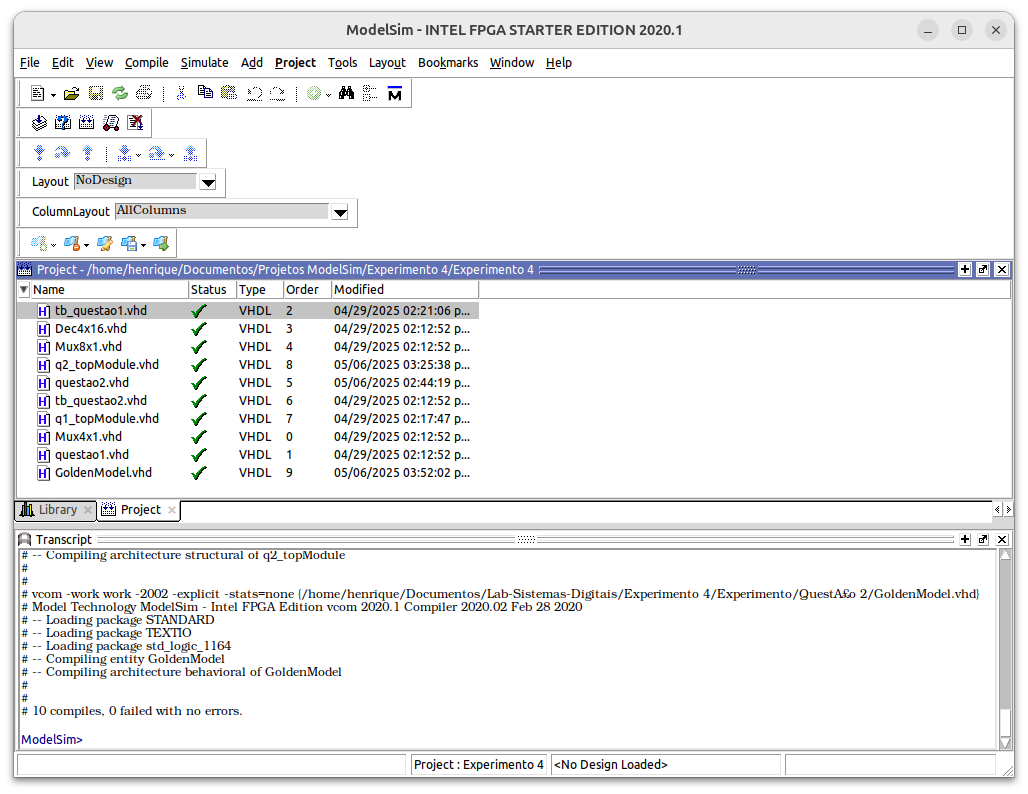
\includegraphics[width=1\textwidth]{Recursos/Imagens/CompileModelSim.png}
    \caption{Compilação de todos os códigos apresentados}
\end{figure}

\newpage

\section{Simulação}
Os gráficos de onda das entradas e saídas dos dispositivos das questões 1 e 2 estão exibidos a seguir. Note que no primeiro, como definido no \textit{testbench}, os sinais de entrada variam a cada 12,5 nanosegundos (ns) no decorrer de 100 ns de simulação, resultando em 8 variações - todas as combinações possíveis dos sinais de entrada. No segundo, as variações ocorrem a cada 1 ns e a simulação dura 128 ns.

\begin{figure}[H]
    \centering
    \begin{tcolorbox}[colframe=cinza, colback=white, boxrule=0.75pt, arc=0pt, width=1\textwidth, center, boxsep=0pt, left=0pt, right=0pt, top=0pt, bottom=0pt]
    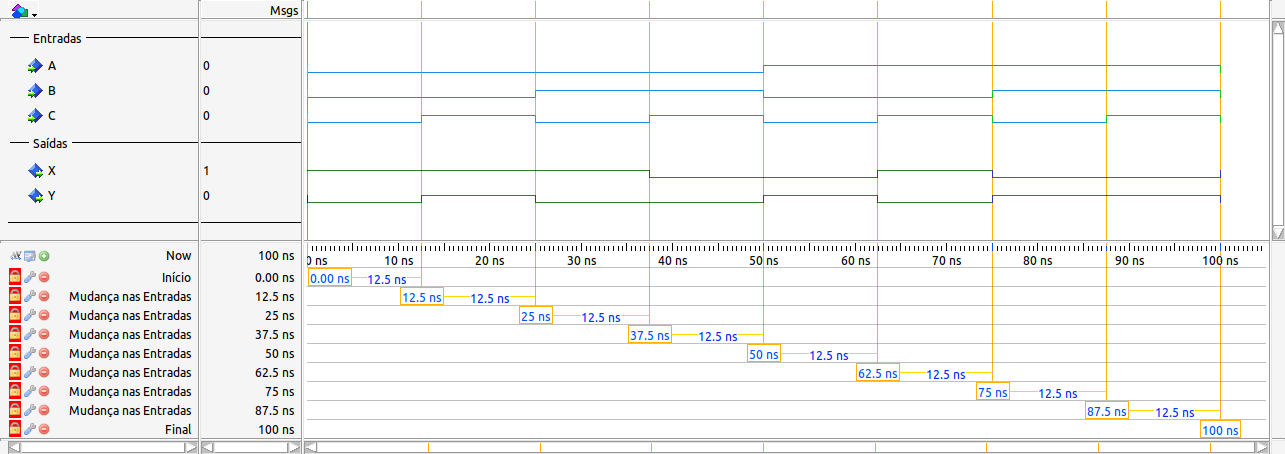
\includegraphics[width=1\textwidth]{Recursos/Imagens/q1.png}
    \end{tcolorbox}
    \caption{Simulação em forma de onda binária do dispositivo da questão 1}
\end{figure}

\begin{figure}[H]
    \centering
    \begin{tcolorbox}[colframe=cinza, colback=white, boxrule=0.75pt, arc=0pt, width=1\textwidth, center, boxsep=0pt, left=0pt, right=0pt, top=0pt, bottom=0pt]
    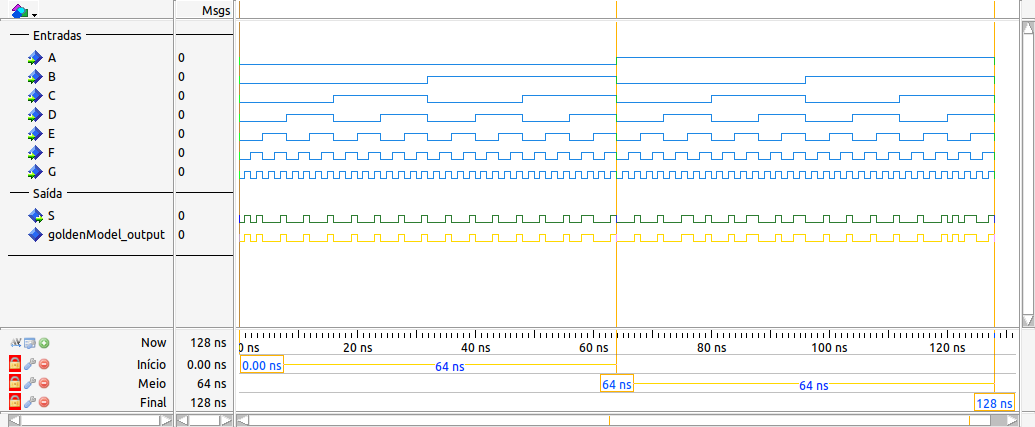
\includegraphics[width=1\textwidth]{Recursos/Imagens/q2.png}
    \end{tcolorbox}
    \caption{Simulação em forma de onda binária do dispositivo da questão 2}
    \label{fig: q2}
\end{figure}

Perceba que, na segunda imagem, há duas ondas de saída. A segunda, em amarelo, representa o \textit{Golden Model}. Note também que, na segunda simulação, não foram colocados cursores a cada variação das entradas. Isso deixaria a imagem muito poluída, então optamos por posicionar cursores apenas no início, meio e fim da simulação.

\newpage

\section{Análise}

\subsection{Questão 1}
O dispositivo da questão 1 tem três entradas e, portanto, oito saídas. Nesse caso, seguiremos o procedimento padrão: exibiremos \textit{prints} das entradas e saídas para cada possível combinação das entradas.

\begin{figure}[H]
    \centering
    \setlength{\lineskip}{5pt} % Remove espaçamento extra entre linhas
\setlength{\baselineskip}{0pt} % Remove espaçamento base entre linhas
% Linha 1 (centralizada)
\begin{minipage}{\textwidth}
    \centering
    \begin{minipage}[t]{0.375\textwidth}
        \begin{tcolorbox}[colframe=cinza, colback=white, boxrule=1pt, arc=0pt, width=\textwidth, boxsep=0pt, left=0pt, right=0pt, top=0pt, bottom=0pt]
            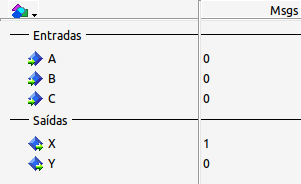
\includegraphics[width=1\textwidth]{Recursos/Imagens/000.png}
        \end{tcolorbox}
    \end{minipage}
    \begin{minipage}[t]{0.375\textwidth}
        \begin{tcolorbox}[colframe=cinza, colback=white, boxrule=1pt, arc=0pt, width=\textwidth, boxsep=0pt, left=0pt, right=0pt, top=0pt, bottom=0pt]
            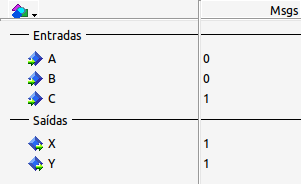
\includegraphics[width=1\textwidth]{Recursos/Imagens/001.png}
        \end{tcolorbox}
    \end{minipage}
\end{minipage}

\begin{minipage}[t]{\textwidth}
    \centering
    \begin{minipage}[t]{0.375\textwidth}
        \begin{tcolorbox}[colframe=cinza, colback=white, boxrule=1pt, arc=0pt, width=\textwidth, boxsep=0pt, left=0pt, right=0pt, top=0pt, bottom=0pt]
            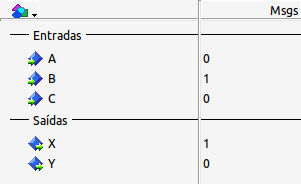
\includegraphics[width=1\textwidth]{Recursos/Imagens/010.png}
        \end{tcolorbox}
    \end{minipage}
    \begin{minipage}[t]{0.375\textwidth}
        \begin{tcolorbox}[colframe=cinza, colback=white, boxrule=1pt, arc=0pt, width=\textwidth, boxsep=0pt, left=0pt, right=0pt, top=0pt, bottom=0pt]
            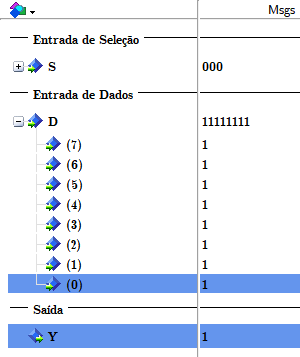
\includegraphics[width=1\textwidth]{Recursos/Imagens/011.png}
        \end{tcolorbox}
    \end{minipage}
\end{minipage}

% Linha 3 (centralizada)
\begin{minipage}{\textwidth}
    \centering
    \begin{minipage}[t]{0.375\textwidth}
        \begin{tcolorbox}[colframe=cinza, colback=white, boxrule=1pt, arc=0pt, width=\textwidth, boxsep=0pt, left=0pt, right=0pt, top=0pt, bottom=0pt]
            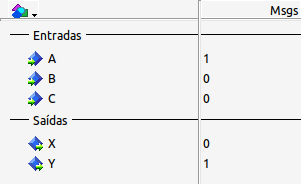
\includegraphics[width=1\textwidth]{Recursos/Imagens/100.png}
        \end{tcolorbox}
    \end{minipage}
    \begin{minipage}[t]{0.375\textwidth}
        \begin{tcolorbox}[colframe=cinza, colback=white, boxrule=1pt, arc=0pt, width=\textwidth, boxsep=0pt, left=0pt, right=0pt, top=0pt, bottom=0pt]
            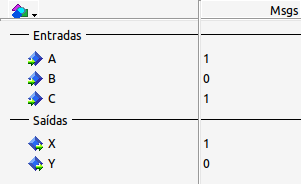
\includegraphics[width=1\textwidth]{Recursos/Imagens/101.png}
        \end{tcolorbox}
    \end{minipage}
\end{minipage}
\begin{minipage}{\textwidth}
    \centering
    \begin{minipage}[t]{0.375\textwidth}
        \begin{tcolorbox}[colframe=cinza, colback=white, boxrule=1pt, arc=0pt, width=\textwidth, boxsep=0pt, left=0pt, right=0pt, top=0pt, bottom=0pt]
            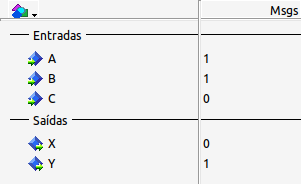
\includegraphics[width=1\textwidth]{Recursos/Imagens/110.png}
        \end{tcolorbox}
    \end{minipage}
    \begin{minipage}[t]{0.375\textwidth}
        \begin{tcolorbox}[colframe=cinza, colback=white, boxrule=1pt, arc=0pt, width=\textwidth, boxsep=0pt, left=0pt, right=0pt, top=0pt, bottom=0pt]
            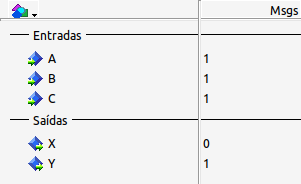
\includegraphics[width=1\textwidth]{Recursos/Imagens/111.png}
        \end{tcolorbox}
    \end{minipage}
\end{minipage}
    \caption{Todas as combinações de entradas do dispositivo da questão 1}
    \label{fig:enter-label}
\end{figure}

Cada \textit{print} na figura acima representa uma linha da tabela-verdade. Comparando o resultado obtido com a \autoref{tab: q1_1}, é evidente que a implementação da questão 1 apresentada está correta. Claro que só consideramos os casos em que as entradas variam entre `0' e `1', os outros valores fornecidos pelo tipo $std\_logic$ são ignorados. Pela implementação do multiplexador, porém, sabemos que a saída seria \textit{don't care} ($-$) em qualquer outro caso.

\subsection{Questão 2}
Na análise da segunda questão, não é necessário (e seria impraticável) exibir os \textit{prints} de todas as possíveis combinações das entradas. Ao invés disso, utilizaremos o \textit{Golden Model}. 
Imediatamente, é fácil perceber que os sinais de saída $S$ e $goldenModel\_output$ são idênticos ao olhar \autoref{fig: q2}, mas, além disso, podemos notar que a mensagem ``Erro!!'' não foi exibida no \textit{Transcript} em nenhum momento da execução, como mostrado no canto inferior da figura a seguir. Dessa forma, fica claro que o dispositivo da questão 2 foi implementado corretamente.

\begin{figure}[H]
    \centering
    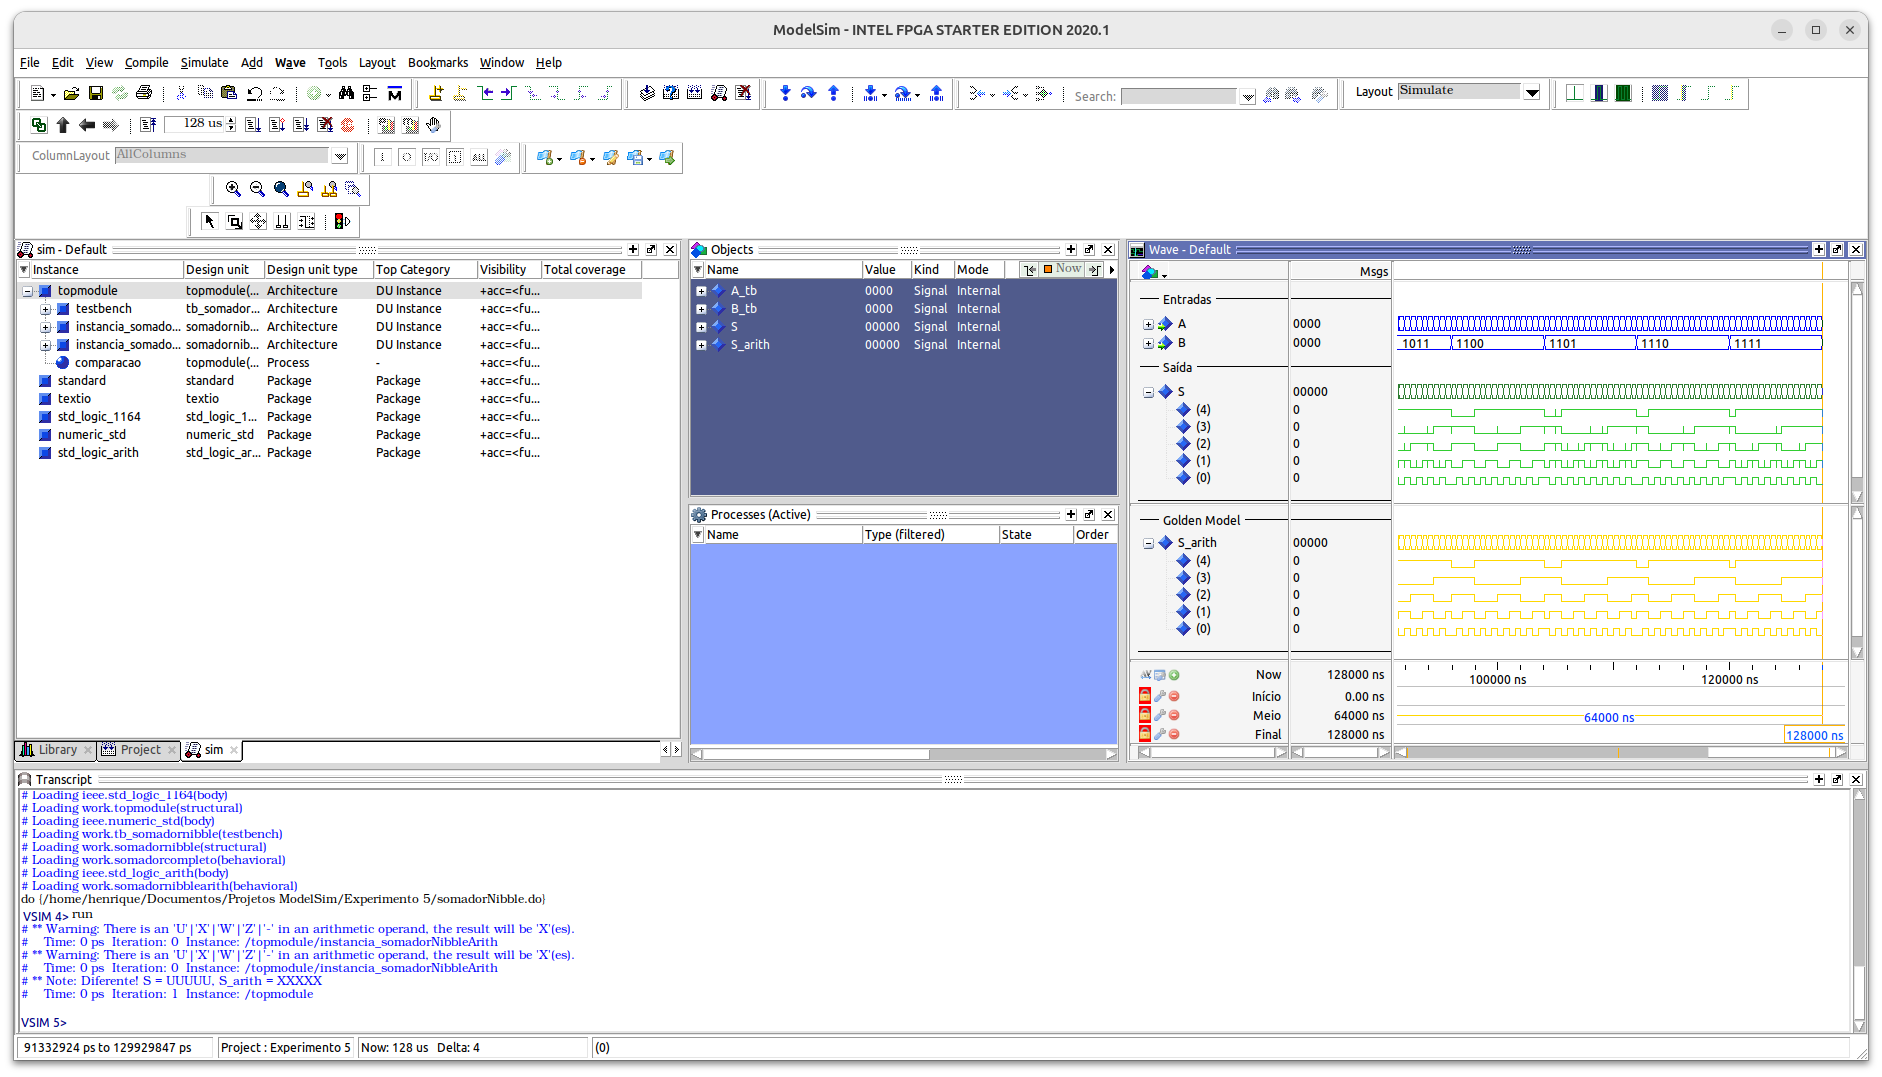
\includegraphics[width=1\linewidth]{Recursos/Imagens/Transcript.png}
    \caption{Tela do ModelSim após a simulação}
\end{figure}

\section{Conclusão}
Nesse experimento, colocamos em prática os conhecimentos sobre multiplexadores e decodificadores explorados nos relatórios anteriores, implementando funções booleanas para descrever a lógica entrada-saída de dois sistemas digitais. Além disso, introduzimos o conceito de \textit{Golden Model} e utilizamos isso para verificar a funcionalidade do sistema da questão 2.

Finalmente, com as práticas introduzidas nesse relatório, conseguimos verificar a correção dos códigos da questão 1 e 2, isto é, verificamos que os sistemas foram devidamente implementados pelos arquivos de descrição de \textit{hardware} apresentados na \autoref{sec: codigos}.

\end{document}